
\documentclass[border=8pt]{standalone}
\def\Conv[\ConvColor]Color{rgb:yellow,5;red,2.5;white,5}
\def\Conv[\ConvColor]ReluColor{rgb:yellow,5;red,5;white,5}
\def\PoolColor{rgb:red,1;black,0.3}
\def\Fc[\FcColor]Color{rgb:blue,5;red,2.5;white,5}
\def\Fc[\FcColor]ReluColor{rgb:blue,5;red,5;white,4}
\def\Softmax[\SoftmaxColor]Color{rgb:magenta,5;black,7}
\usepackage{tikz}
\usepackage{verbatim}
\usepackage{adjustbox}
\usepackage[utf8]{inputenc}
\usepackage{amsmath}
\usepackage{graphicx}
\usepackage{pgfplots}
\usepackage{tikz-3dplot}
\usepackage{tikz-cd}

\usetikzlibrary{positioning}
\usetikzlibrary{shapes.geometric}
\usetikzlibrary{fit,calc}
\usetikzlibrary{3d}

\tikzset{
    conv/.style={draw, fill=blue!20, minimum width=1.2cm, minimum height=1.8cm},
    downsample/.style={draw, fill=purple!20, minimum width=1.2cm, minimum height=1.2cm},
    leakyrelu/.style={draw, fill=orange!30, minimum width=1.2cm, minimum height=0.8cm},
    linear/.style={draw, fill=green!30, minimum width=1.2cm, minimum height=1cm},
    skip/.style={->, thick},
    block/.style={draw, dashed, rounded corners, inner sep=5pt}
}

\begin{document}
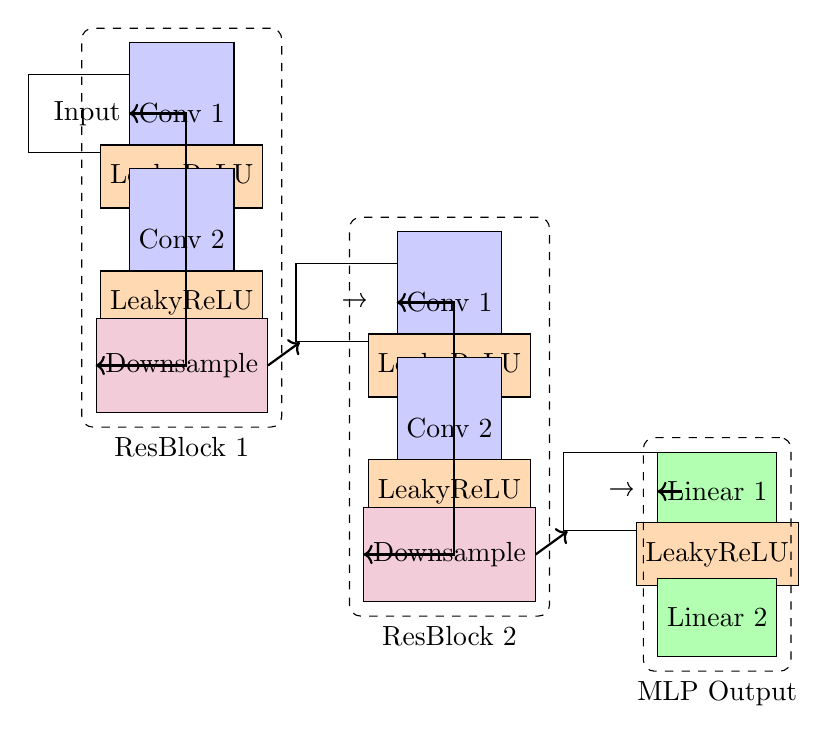
\begin{tikzpicture}[node distance=0.8cm and 1.2cm, on grid]

% Input
\node[draw, minimum width=1.5cm, minimum height=1cm] (input) {Input};

% ResBlock 1
\node[conv, right=of input] (conv1a) {Conv 1};
\node[leakyrelu, below=of conv1a] (relu1a) {LeakyReLU};
\node[conv, below=of relu1a] (conv1b) {Conv 2};
\node[leakyrelu, below=of conv1b] (relu1b) {LeakyReLU};
\node[downsample, below=of relu1b] (down1) {Downsample};

\node[block, fit=(conv1a) (down1), label=below:{ResBlock 1}] (block1) {};

% Skip Connection
\draw[skip] (input.east) -- ++(0.5,0) |- (down1.west);

% Output from ResBlock 1
\node[draw, minimum width=1.5cm, minimum height=1cm, right=2.2cm of relu1b] (res1_out) {→};

% ResBlock 2
\node[conv, right=of res1_out] (conv2a) {Conv 1};
\node[leakyrelu, below=of conv2a] (relu2a) {LeakyReLU};
\node[conv, below=of relu2a] (conv2b) {Conv 2};
\node[leakyrelu, below=of conv2b] (relu2b) {LeakyReLU};
\node[downsample, below=of relu2b] (down2) {Downsample};

\node[block, fit=(conv2a) (down2), label=below:{ResBlock 2}] (block2) {};

% Skip Connection 2
\draw[skip] (res1_out.east) -- ++(0.5,0) |- (down2.west);

% Output from ResBlock 2
\node[draw, minimum width=1.5cm, minimum height=1cm, right=2.2cm of relu2b] (res2_out) {→};

% Final Linear Layers
\node[linear, right=of res2_out] (linear1) {Linear 1};
\node[leakyrelu, below=of linear1] (relu_lin) {LeakyReLU};
\node[linear, below=of relu_lin] (linear2) {Linear 2};

\node[block, fit=(linear1) (linear2), label=below:{MLP Output}] (mlpblock) {};

% Arrows
\draw[->, thick] (input) -- (conv1a);
\draw[->, thick] (down1.east) -- (res1_out);
\draw[->, thick] (res1_out) -- (conv2a);
\draw[->, thick] (down2.east) -- (res2_out);
\draw[->, thick] (res2_out) -- (linear1);

\end{tikzpicture}
\end{document}